\documentclass[UTF8]{ctexart}
\usepackage{geometry}
\usepackage[backend=biber, style=authoryear]{biblatex} % 示例配置
\addbibresource{references.bib} % 替换为你的参考文献文件
\geometry{margin=1.5cm, vmargin={0pt,1cm}}
\setlength{\topmargin}{-1cm}
\setlength{\paperheight}{29.7cm}
\setlength{\textheight}{25.3cm}

% useful packages.
\usepackage{amsfonts}
\usepackage{amsmath}
\usepackage{amssymb}
\usepackage{amsthm}
\usepackage{enumerate}
\usepackage{graphicx}
\usepackage{multicol}
\usepackage{fancyhdr}
\usepackage{layout}
\usepackage{listings}
\usepackage{xcolor}
%\lstset{language=C++}
\setlength{\headheight}{13pt}  % 增加头部高度
\usepackage{float, caption}

% Listings setting for code formatting
\lstset{
    basicstyle=\ttfamily,
    keywordstyle=\color{blue},
    commentstyle=\color{gray},
    stringstyle=\color{red},
    breaklines=true,
    frame=single,
    numbers=left,
    numberstyle=\tiny,
    stepnumber=1,
    tabsize=4,
}

% some common commands
\newcommand{\dif}{\mathrm{d}}
\newcommand{\avg}[1]{\left\langle #1 \right\rangle}
\newcommand{\difFrac}[2]{\frac{\dif #1}{\dif #2}}
\newcommand{\pdfFrac}[2]{\frac{\partial #1}{\partial #2}}
\newcommand{\OFL}{\mathrm{OFL}}
\newcommand{\UFL}{\mathrm{UFL}}
\newcommand{\fl}{\mathrm{fl}}
\newcommand{\op}{\odot}
\newcommand{\Eabs}{E_{\mathrm{abs}}}
\newcommand{\Erel}{E_{\mathrm{rel}}}

\begin{document}

\pagestyle{fancy}
\fancyhead{}
\lhead{陈梓锐}
\chead{22435036}
\rhead{\today}


%\begin{abstract}
 %   The abstract is not necessary for the theoretical homework, 
   % but for the programming project, 
    %you are encouraged to write one.      
%\end{abstract}

% ============================================

\subsection*{Exercise 10.14}
考虑两个IVPs
$
\left\{
\begin{aligned}
v^{'} &= f(v,t) \\
v(a) &= v_0  
\end{aligned}
\right.
$和
$
\left\{
\begin{aligned}
w^{'} &= f(u,t) \\  
w(a) &= 0  
\end{aligned}
\right.
$,
显然IVPs解分别为$v(t) = v_0 + \int_{a}^{t} f(v,s) d s$和$w(t) = w_0 + \int_a^t f(w(s),s) d s$.
\begin{align*}
    \|v(t) - w(t)\| &= \|v_0 -w_0\| + \| \int_{a}^{t} f(v,s) - f(w(s),s) d s \| \\
                    &\leq \|v_0 -w_0\| + \int_{a}^{t} \|f(v,s) - f(w(s),s)\| d s \\
                    &\leq \|v_0 - w_0\| + \int_{a}^{t} L\|v(s) - w(s) \| ds
\end{align*}
由Gronwall不等式，

$\Rightarrow \|v(t) - w(t)\| \leq \|v_0 - w_0\|\cdot exp\{\int_{a}^{t} L ds\} = \|v_0 - w_0\| \cdot exp\{L(t-a)\}$.


\subsection*{Exercise 10.64}
Trapezoidal:
$$C_0 = 0, C_1 = 0, C_2 = -1, C_3 = -\frac{1}{12}, C_4 = -\frac{1}{24}$$
Midpoint:
$$C_0 = 0, C_1 = 0, C_2 = 0, C_3 = \frac{1}{3}, C_4 = \frac{1}{3}$$

\subsection*{Exercise 10.66}
为了达到3阶精度，需令$C_0 = C_1 = C_2 = 0$, 即
$$\sum_{n = 0}^{s} a_n = 0, \quad \sum_{n = 0}^{s} na_n = \sum_{n = 0}^{s} b_n, \quad \sum_{n = 0}^{s} n^2a_n = \sum_{n = 0}^{s} nb_n$$.
即$\rho(1) = 0, \rho^{'}(1) = \sigma (1), \rho^{'}(1) + \rho^{''}(1) = \frac{1}{2}\sigma^{'}(1)$.

\subsection*{Exercise 10.67}
Adams-Bashforth方法：

s步显式方法，系数通过积分拉格朗日插值多项式获得。

\begin{lstlisting}[language=Matlab, caption={MATLAB 示例代码}, label=code:matlab]
syms theta;
s = input('Enter the value of s: ');
theta_nodes = 0 : -1 : -(s-1); 
beta = zeros(1, s);

for i = 0 : s-1
    current_theta = theta_nodes(i+1);
    Li = 1;
    for k = 0 : s-1
        if k ~= i
            Li = Li * (theta - theta_nodes(k+1)) / (current_theta - theta_nodes(k+1));
        end
    end
    beta(i+1) = int(Li, theta, 0, 1);
end

disp('Coefficients (from beta_s-1 to beta_0):');
disp(vpa(beta, 4));
\end{lstlisting}

Coefficients: [3/2, -1/2]

Coefficients: [23/12, -4/3, 5/12]

Coefficients: [55/24, -59/24, 37/24, -3/8]

%============================================================
Adams-Moulton:

隐式多步法，其系数通过积分拉格朗日插值多项式得到。其插值节点包含当前时刻 $t_{n+1}$.
\begin{lstlisting}
syms theta;
s = input('Enter the value of s (Adams-Moulton): ');
theta_nodes = 0 : -1 : -(s-1);
beta = zeros(1, s);

for i = 0 : s-1
    current_theta = theta_nodes(i+1);
    Li = 1;
    for k = 0 : s-1
        if k ~= i
            Li = Li * (theta - theta_nodes(k+1)) / (current_theta - theta_nodes(k+1));
        end
    end
    beta(i+1) = int(Li, theta, 0, 1); 
end

disp('Adams-Moulton Coefficients (\beta_s 到 \beta_0):');
disp(vpa(beta, 4));
\end{lstlisting}

Coefficients: [1/2, 1/2]

Coefficients: [5/12, 8/12, -1/12]

Coefficients: [9/24, 19/24, -5/24, 1/24]

%============================================================
BDF:

隐式方法，通过多项式插值并强制导数条件确定系数。

\begin{lstlisting}
syms h t;
s = input('Enter the value of s (BDF): ');
a = sym('a', [1, s+1]);
p = sum(a .* t.^(0:s));

eqns = [];
for k = 1:s
    eqns = [eqns, subs(p, t, -k*h) == 0];
end

dpdt = diff(p, t);
eqns = [eqns, subs(dpdt, t, 0) == 1]; 

[A, B] = equationsToMatrix(eqns, a);
sol = linsolve(A, B);

alpha = [1; -double(sol(2:end))];
beta = 1; 

disp(vpa(alpha.', 4));
disp(vpa(beta, 4));
\end{lstlisting}

$\alpha: [1, -1], \beta: 1$

$\alpha: [1, -4/3, 1/3], \beta: 2/3$

$\alpha: [1, -18/11, 9/11, -2/11], \beta: 6/11$


\subsection*{Exercise 10.72}
$\rho(z) = \sum_{j = 0}^{3} \alpha_j z^j = Z^3 -\frac{18}{11}z^2 + \frac{9}{11}z - \frac{2}{11}$,

$\sigma (z) = \sum_{j = 0}^{3} \beta_j z^j = \frac{6}{11}z^3$,

$g(z) = \frac{\rho(z)}{\sigma(z)} = \frac{11}{6} - \frac{3}{z} + \frac{3}{2z^2} - \frac{1}{3z^3}$.

$g(1) = 0, g^{'}(1) = -1, g^{''}(1) = 2, g^{(4)}(1) = -12$.

在z=1处展开：

$g(z) = (z-1) - \frac{1}{2}(z-1)^2 + \frac{1}{3}(z-1)^3 -\frac{1}{4}(z-1)^4 + \varTheta (-\frac{1}{4}(z-1)^4)$.


\subsection*{Exercise 10.73}
由（10.44）$L_u(t_n) = C_0u(t_n) + C_1ku_t(t_n) + C_2k^2u_{tt}(t_n) + \cdots$

必要性：

假设LMM有p阶精度，$\forall j = 0,1,\cdots,p$有$C_j = 0, C_{p+1} \neq 0$.若$q(t)$阶数小于p，则$\forall j = p, p+1, \cdots$
有$\frac{\partial^j}{\partial t^j}q(t) = \frac{\partial^{j+1}}{\partial t^{j+1}}u = 0$.
此时$L_u(t_n) = 0$,又因为已知初始条件精确，所以解完全精确。

充分性：

$L_u(t_n) = C_0u(t_n) + \sum_{j = 1}^{\infty} C_jk^jq^{(j-1)}(t_n)$

因为$\forall q(t)$是p-1阶多项式，所以$L_u(t_n) = 0$, 

取$q(t) = 0 \Rightarrow C_0 = 0,\quad q(t) = t \Rightarrow C_1 = 0,\cdots,q(t) = t^{p-1}\Rightarrow C_{p} = 0$.

当q阶数大于p-1时，不妨设$q(t) = t^p$, 此时$L_u(t_n) \neq 0$,即$C_{p+1} \neq 0$,则$L_u(t_n)$为p阶精度。

\subsection*{Exercise 10.82}
当$n = 0,1,\cdots,s-1时$
$
\begin{pmatrix}
    y_{s-1} \\
    y_{s-2} \\
    \vdots \\
    y_1 \\
    y_0
\end{pmatrix}
$=$\begin{pmatrix}
    1 &\theta_1 &\theta_2 &\cdots &\theta_{s-1} \\
    0 &1 &\theta_1 &\cdots &\theta_{s-2} \\
    \vdots &\vdots &\vdots &\vdots &\vdots \\
    0 &0 &\cdots &1 &\theta_1\\
    0 &0 &\cdots &0 &1 
\end{pmatrix}$,
$\begin{pmatrix}
    \hat{y_{s-1}} \\
    \hat{y_{s-2}} \\
    \vdots \\
    \hat{y_1} \\
    \hat{y_0}
\end{pmatrix}$

即$y_n = \sum_{i = 0}^{s-1}\theta_{n-i}\hat{y_i}$.

当n > s时，归纳假设(10.62)对$\forall n =  m+s-1$成立，下证对n=m+s-1成立。由已知条件
$y_{n+s} = \phi_{n+s} - \sum_{i = 0}^{s-1}\alpha_iy_{n+i}, \theta_{n+s} + \sum_{i = 0}^{s-1}\alpha_i\theta_{n+i} = 0$.
由归纳假设$y_{n+i} = \sum_{j = 0}^{s-1}\theta_{n+i-j}\hat{y_j} + \sum_{j = s}^{n+i}\theta_{n+i-j}\hat{\phi_j}$,
\begin{align*}
    \Rightarrow y_{n+s} &= \phi_{n+s} - \sum_{i = 0}^{s-1}\alpha_i(\sum_{j = 1}^{s-1}\theta_{n+i-j}\hat{y_j}
                         + \sum_{j=s}^{n+i}\theta_{n+i-j}\phi_j) \\
                        &= \phi_{n+s} - \sum_{i = 0}^{s-1} \hat{y_j}\sum_{i=0}^{s-1}\alpha_i\theta_{n+i-j}
                         + \sum_{j=s}^{n+i}\phi_j\sum_{i = 0}^{s-1}\alpha_i\theta_{n+i-j} \\
                        &= \phi_{n+s} + \sum_{j=0}^{s-1}\theta_{n+s-j}\hat{y_j} + \sum_{j=s}^{n+s-1}\theta_{n+s-j}\phi_j \\
                        &= \sum_{j=0}^{s-1}\theta_{n+s-j}\hat{y_j} + \sum_{j=s}^{n+s-1}\theta_{n+s-j}\phi_j
\end{align*}
令n+s = n即所欲证式。

\subsection*{Exercise 10.87}
考虑IVPS:$u^{'} = f(t) = 0, u(0) = 1$,真解为1.

LMM方法：$\sum_{j=0}^{s}\alpha_jU^{n+j} = 0$
因为收敛，所以初值满足$\lim_{k \to 0} U^j = 1,j = 0,1,\cdots,s-1$，解满足$ \lim_{k \to 0, Nk = t} U^{N} = 1$.

则对$\sum_{j=0}^{s}\alpha_jU^{n+j} = 0$中k取极限0，有$\sum_{j=0}^{s}\alpha_j = 0$，则LMM满足preconsistent。


考虑IVPS:$u^{'} = f(t) = 1, u(0) = 0$,真解为1.

LMM方法：$\sum_{j=0}^{s}\alpha_jU^{n+j} = k\sum_{j=0}^{s}\beta_j$
因为收敛，所以初值满足$\lim_{k \to 0} U^j = 0,j = 0,1,\cdots,s-1$，解满足$ \lim_{k \to 0, Nk = t} U^{N} = t$.

则对$\sum_{j=0}^{s}\alpha_jU^{n+j} = k\sum_{j=0}^{s}\beta_j$两边同时对k取极限0，因为Nk=t,有$\sum_{j=0}^{s}j\alpha_j = \sum_{j=0}^{s}\beta_j$，
则LMM满足consistent。


\subsection*{Exercise 10.102}
Adams-Bashforth 方法
\begin{lstlisting}
import numpy as np
import matplotlib.pyplot as plt

orders = [1, 2, 3, 4, 5]
theta = np.linspace(0, 2 * np.pi, 1000)
z = np.exp(1j * theta)

plt.figure(figsize=(10, 6))
plt.title("Adams-Bashforth 绝对稳定域 (p=1 到 5)")
plt.xlabel("Re(κ)")
plt.ylabel("Im(κ)")
plt.grid(True)

for p in orders:
    if p == 1:
        rho_coeff = [1, -1]        
        sigma_coeff = [0, 1]       
    elif p == 2:
        rho_coeff = [1, -1, 0]     
        sigma_coeff = [0, 3/2, -1/2]
    elif p == 3:
        rho_coeff = [1, -1, 0, 0]
        sigma_coeff = [0, 23/12, -16/12, 5/12]
    elif p == 4:
        rho_coeff = [1, -1, 0, 0, 0]
        sigma_coeff = [0, 55/24, -59/24, 37/24, -9/24]
    elif p == 5:
        rho_coeff = [1, -1, 0, 0, 0, 0]
        sigma_coeff = [0, 1901/720, -2774/720, 2616/720, -1274/720, 251/720]

    rho = np.polyval(rho_coeff, z)
    sigma = np.polyval(sigma_coeff, z)
    gamma = rho / sigma

    plt.plot(np.real(gamma), np.imag(gamma), label=f"p={p}")

plt.legend()
plt.show()
\end{lstlisting}
\begin{figure}[H]
    \centering
    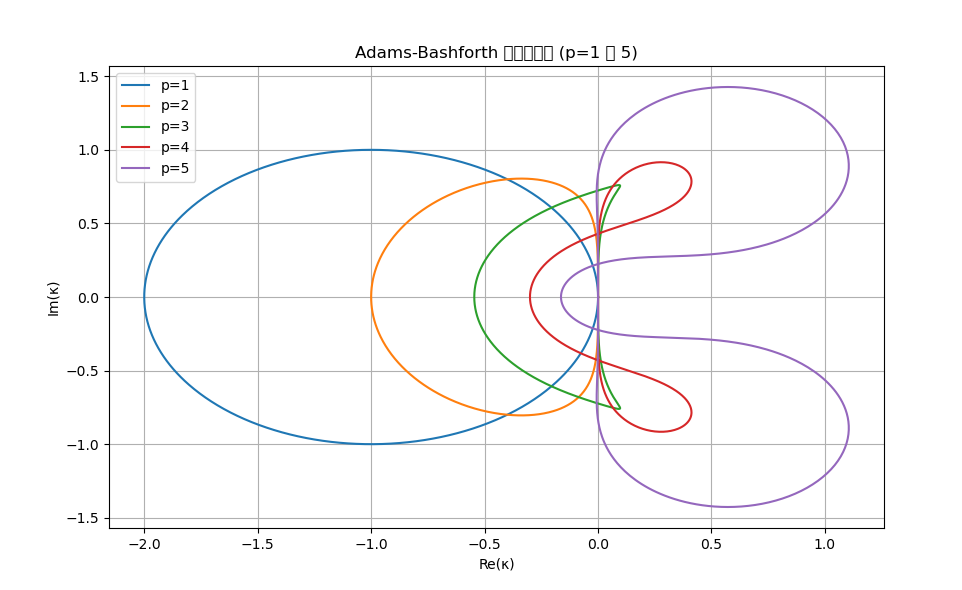
\includegraphics[width=0.8\textwidth]{AB.png}
    \caption{Adams-Bashforth 绝对稳定域 (p=1 到 5)}
\end{figure}

Adams-Moulton 方法
\begin{lstlisting}import numpy as np
    import matplotlib.pyplot as plt
    
    orders = [3, 4, 5]
    theta = np.linspace(0, 2 * np.pi, 1000)
    z = np.exp(1j * theta)
    
    plt.figure(figsize=(10, 6))
    plt.title("Adams-Moulton 绝对稳定域 (p=3 到 5)")
    plt.xlabel("Re(κ)")
    plt.ylabel("Im(κ)")
    plt.grid(True)
    
    for p in orders:
        if p == 3:
            rho_coeff = [1, -1, 0, 0]
            sigma_coeff = [5/12, 2/3, -1/12, 0]
        elif p == 4:
            rho_coeff = [1, -1, 0, 0, 0]
            sigma_coeff = [3/8, 19/24, -5/24, 1/24, 0]
        elif p == 5:
            rho_coeff = [1, -1, 0, 0, 0, 0]
            sigma_coeff = [251/720, 646/720, -264/720, 106/720, -19/720, 0]
        
        rho = np.polyval(rho_coeff, z)
        sigma = np.polyval(sigma_coeff, z)
        gamma = rho / sigma
    
        plt.plot(np.real(gamma), np.imag(gamma), label="p={}".format(p))
    
    plt.legend()
    plt.show()
    
\end{lstlisting}
\begin{figure}[H]
    \centering
    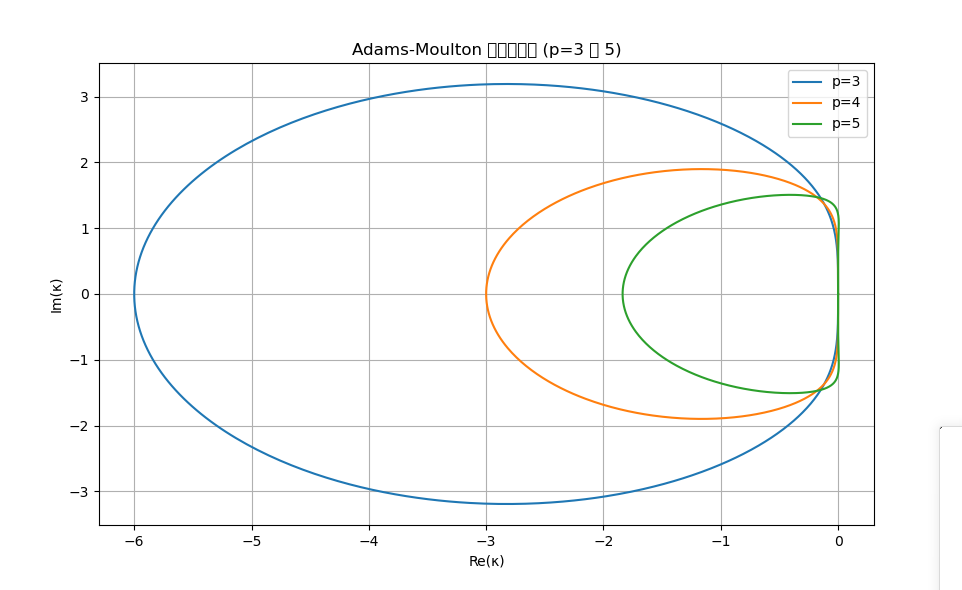
\includegraphics[width=0.8\textwidth]{AM.png}
    \caption{Adams-Moulton 绝对稳定域 (p=3 到 5)}
\end{figure}





BDF 方法
\begin{lstlisting}
import numpy as np
import matplotlib.pyplot as plt

orders = [3, 4, 5]
theta = np.linspace(0, 2 * np.pi, 1000)
z = np.exp(1j * theta)

plt.figure(figsize=(10, 6))
plt.title("Adams-Moulton 绝对稳定域 (p=3 到 5)")
plt.xlabel("Re(κ)")
plt.ylabel("Im(κ)")
plt.grid(True)

for p in orders:
    if p == 3:
        rho_coeff = [1, -1, 0, 0]
        sigma_coeff = [5/12, 2/3, -1/12, 0]
    elif p == 4:
        rho_coeff = [1, -1, 0, 0, 0]
        sigma_coeff = [3/8, 19/24, -5/24, 1/24, 0]
    elif p == 5:
        rho_coeff = [1, -1, 0, 0, 0, 0]
        sigma_coeff = [251/720, 646/720, -264/720, 106/720, -19/720, 0]
    
    rho = np.polyval(rho_coeff, z)
    sigma = np.polyval(sigma_coeff, z)
    gamma = rho / sigma

    plt.plot(np.real(gamma), np.imag(gamma), label="p={}".format(p))

plt.legend()
plt.show()

\end{lstlisting}

\begin{figure}[H]
    \centering
    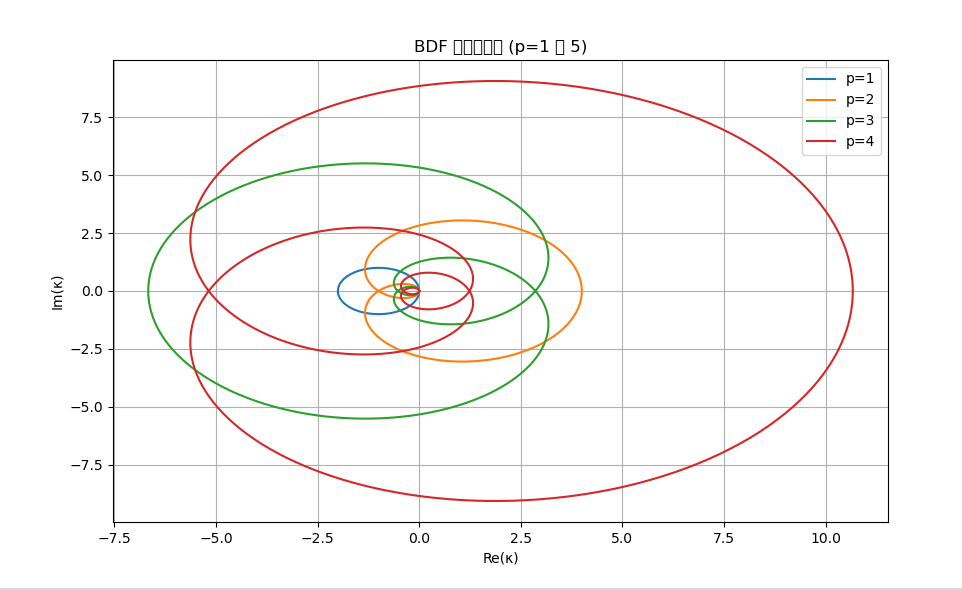
\includegraphics[width=0.8\textwidth]{BDF.png}
    \caption{BDF 绝对稳定域 (p=3 到 5)}
\end{figure}
















% ===============================================

\end{document}